\documentclass[12pt,a4paper]{article}
\usepackage[margin=1in]{geometry}
\usepackage[utf8]{inputenc}
\usepackage{amsmath}
\usepackage{amsfonts}
\usepackage{amssymb}
\usepackage{graphicx}
\usepackage{enumerate}
\usepackage{bm}
\usepackage{pythonhighlight}
\usepackage{fontspec}
\usepackage{xeCJK}
\setCJKmainfont{SimSun}
\usepackage{tikz}
\usetikzlibrary{arrows,positioning}
\usepackage{float}

\geometry{left=1.00in,right=1.00in,top=1.00in,bottom=1.00in}

\title{homework 3}
\author{Zuyao Chen 201728008629002}
\date{}
\begin{document}
\maketitle
\section{Problem 1}
\textbf{Q: } 
设有如下三类模式样本集$w_1$,$w_2$和$w_3$,其先验概率相等,求$S_w$和$S_b$
\[
	\begin{split}
		w_1:& (1,0)^T, (2,0)^T, (1,1)^T  \\
		w_2:& (-1,0)^T, (0,1)^T, (-1,1)^T   \\
		w_3:& (-1,-1)^T, (0,-1)^T, (0,-2)^T \\
	\end{split}
\]
\textbf{A: }
先验概率相等, $P(w) = 1/3$,  均值和协方差矩阵为
\[
	\begin{split}
	 m_1 &= (\frac{4}{3}, \frac{1}{3})^T, m_2 = (-\frac{2}{3},   	\frac{2}{3})^T, m_3 = (-\frac{1}{3}, -\frac{4}{3})^T \\
	 C_1 &= E[(x-m_1)(x-m_1)^T] = \frac{1}{3} \left(\begin{array}{cc} 
		 \frac{2}{3} & -\frac{1}{3} \\
		 -\frac{1}{3} & \frac{2}{3}
	 \end{array} \right)  \\
	 C_2 &= E[(x-m_2)(x-m_2)^T] = \frac{1}{3} \left(\begin{array}{cc} 
	 \frac{2}{3} & \frac{1}{3} \\
	 \frac{1}{3} & \frac{2}{3}
	 \end{array} \right)  \\
	 C_3 &= E[(x-m_3)(x-m_3)^T] = \frac{1}{3} \left(\begin{array}{cc} 
	 \frac{2}{3} & -\frac{1}{3} \\
	 -\frac{1}{3} & \frac{2}{3}
	 \end{array} \right)  \\	 
	\end{split}
\]
因此
\[
	\begin{split} 
	S_w &= \sum_{i=1}^{3}P(w_i)C_i  \\
		&= \frac{1}{9} \left(\begin{array}{cc}
			2 & -1 \\
			-1 & 2
		\end{array} \right) \\
	\end{split} 	
\]
 \[ \begin{split} 
	 m_0 &= \sum_{i=1}^{3} P(w_i)m_i =  (\frac{1}{9}, -\frac{1}{9})^T \\
	 S_b &= \sum_{i=1}^{3} P(w_i)(m_i - m_0)(m_i - m_0)^T \\
		 &= \frac{1}{3} [	
			 (\frac{11}{9},\frac{4}{9})^T(\frac{11}{9},\frac{4}{9}) 
			+ (\frac{-7}{9},\frac{7}{9})^T (\frac{-7}{9},\frac{7}{9}) 
			+(\frac{-4}{9},\frac{-11}{9})^T(\frac{-4}{9},\frac{-11}{9}) 
		 ] \\
		 &= \frac{1}{81} \left(\begin{array}{cc}
			62 & 13 \\
			13 & 62
		 \end{array} \right) 
	\end{split}  
 \]

\section{Problem 2}
\textbf{Q: }设有如下两类样本集,其出现的概率相等: 
\[
	\begin{split}
		w_1:&\{(0,0,0)^T, (2,0,0)^T, (2,0,1)^T, (1,2,0)^T\}  \\
		w_2:&\{(0,0,1)^T, (0,1,0)^T, (0,-2,1)^T, (1,1,-2)^T\}  
	\end{split}
\]
用K-L变换,分别把特征空间维数降到二维和一维,并画出样本在该空间中的位置(可用matlab计算). \\
\textbf{A: } 
 样本均值为$m = (0.75, 0.25, 0.125)^T$, 将所有样本减去均值得到新的样本集为
 \[
	 \begin{split} 
	 w_1:& (-0.75, -0.25, -0.125)^T, (1.25,-0.25,-0.125)^T,(1.25,-0.25,0.875)^T,(0.25,1.75,-0.125)^T \\
	 w_2:& (-0.75,-0.25,0.875)^T, (-0.75,0.75, -0.125)^T, (-0.75,-2.25,0.875)^T,(0.25,0.75,-2.125)^T
	 \end{split} 
 \]
\[
	R = \sum_{i=1}^{2}P(w_i)E(xx^T) = \left(\begin{array}{ccc}
	 0.6875 &   0.1875 &  -0.09375  \\
	  0.1875 &   1.1875&   -0.53125 \\
	 -0.09375&  -0.53125&   0.859375\\
	 \end{array}\right) 
\]
求解$R$的特征值和特征向量,$\lambda_1 = 1.625,\lambda_2= 0.64876246,\lambda_3 = 0.46061254$,对应的一个特征向量组
\[	\begin{split} 
	\phi_1 &= (0.21538745,0.78975397, -0.57436653 )^T, \\
	\phi_2 &= (0.95853318,-0.05858624,0.27889386 )^T,  \\
	\phi_3 &= (-0.18660756,0.61061961,0.76962413)^T
	\end{split} 
\]
选取$\lambda_1,\lambda_2$对应的特征向量作为变换矩阵, 由$ y = (\phi_1,\phi_2)^Tx$得到变换后的二维模式特征为
\[ \begin{split} 
	w_1: &(0,0)^T, (0.4307749,1.91706637)^T, (-0.14359163,2.19596023)^T, (1.7948954,0.8413607)^T \\
	w_2: &(-0.57436653, 0.27889386)^T, (0.78975397,-0.05858624)^T, \\ &(-2.15387448,0.39606634)^T, (2.15387448,0.34215922)^T	
	\end{split} 
\]
选择$\lambda_1$对应的特征向量作为变换矩阵,由$y = \phi_1^Tx$得到一维的模式特征为
\[
	\begin{split} 
	w_1: & 0.        ,  0.4307749 , -0.14359163,  1.7948954\\
	w_2: &-0.57436653, 0.78975397, -2.15387448,  2.15387448 
	\end{split} 	
\]
原始数据的空间分布图如下
\begin{figure}[H]
	\centering
	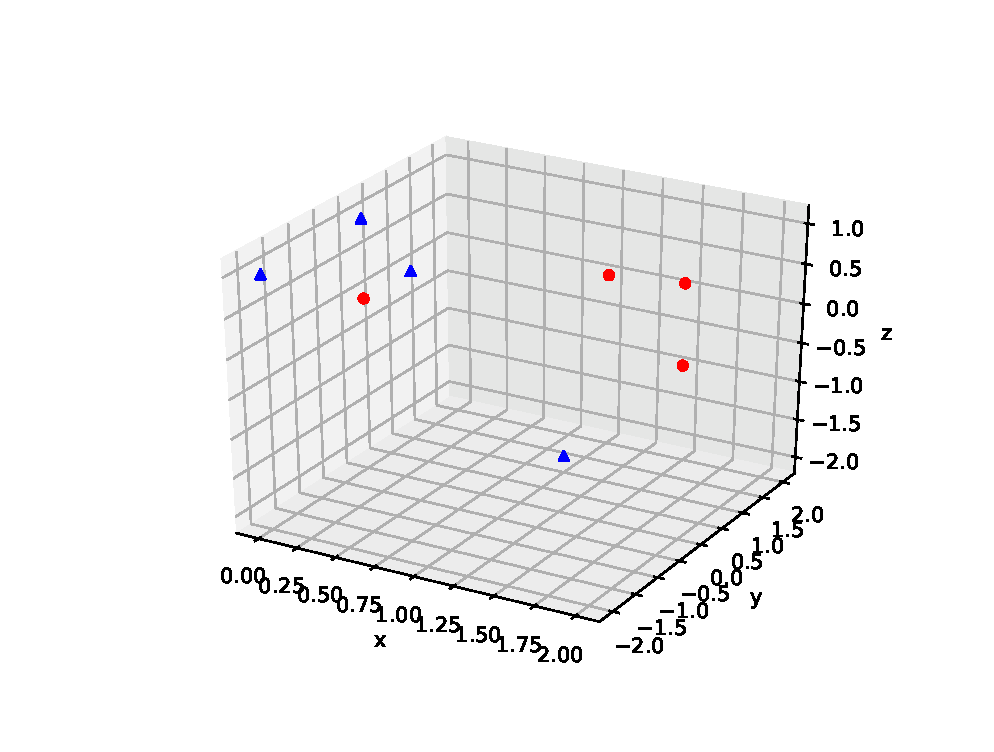
\includegraphics[width = 0.6\textwidth,height=0.3\textheight]{raw}
\end{figure} 
降到二维的空间分布
\begin{figure}[H]
	\centering
	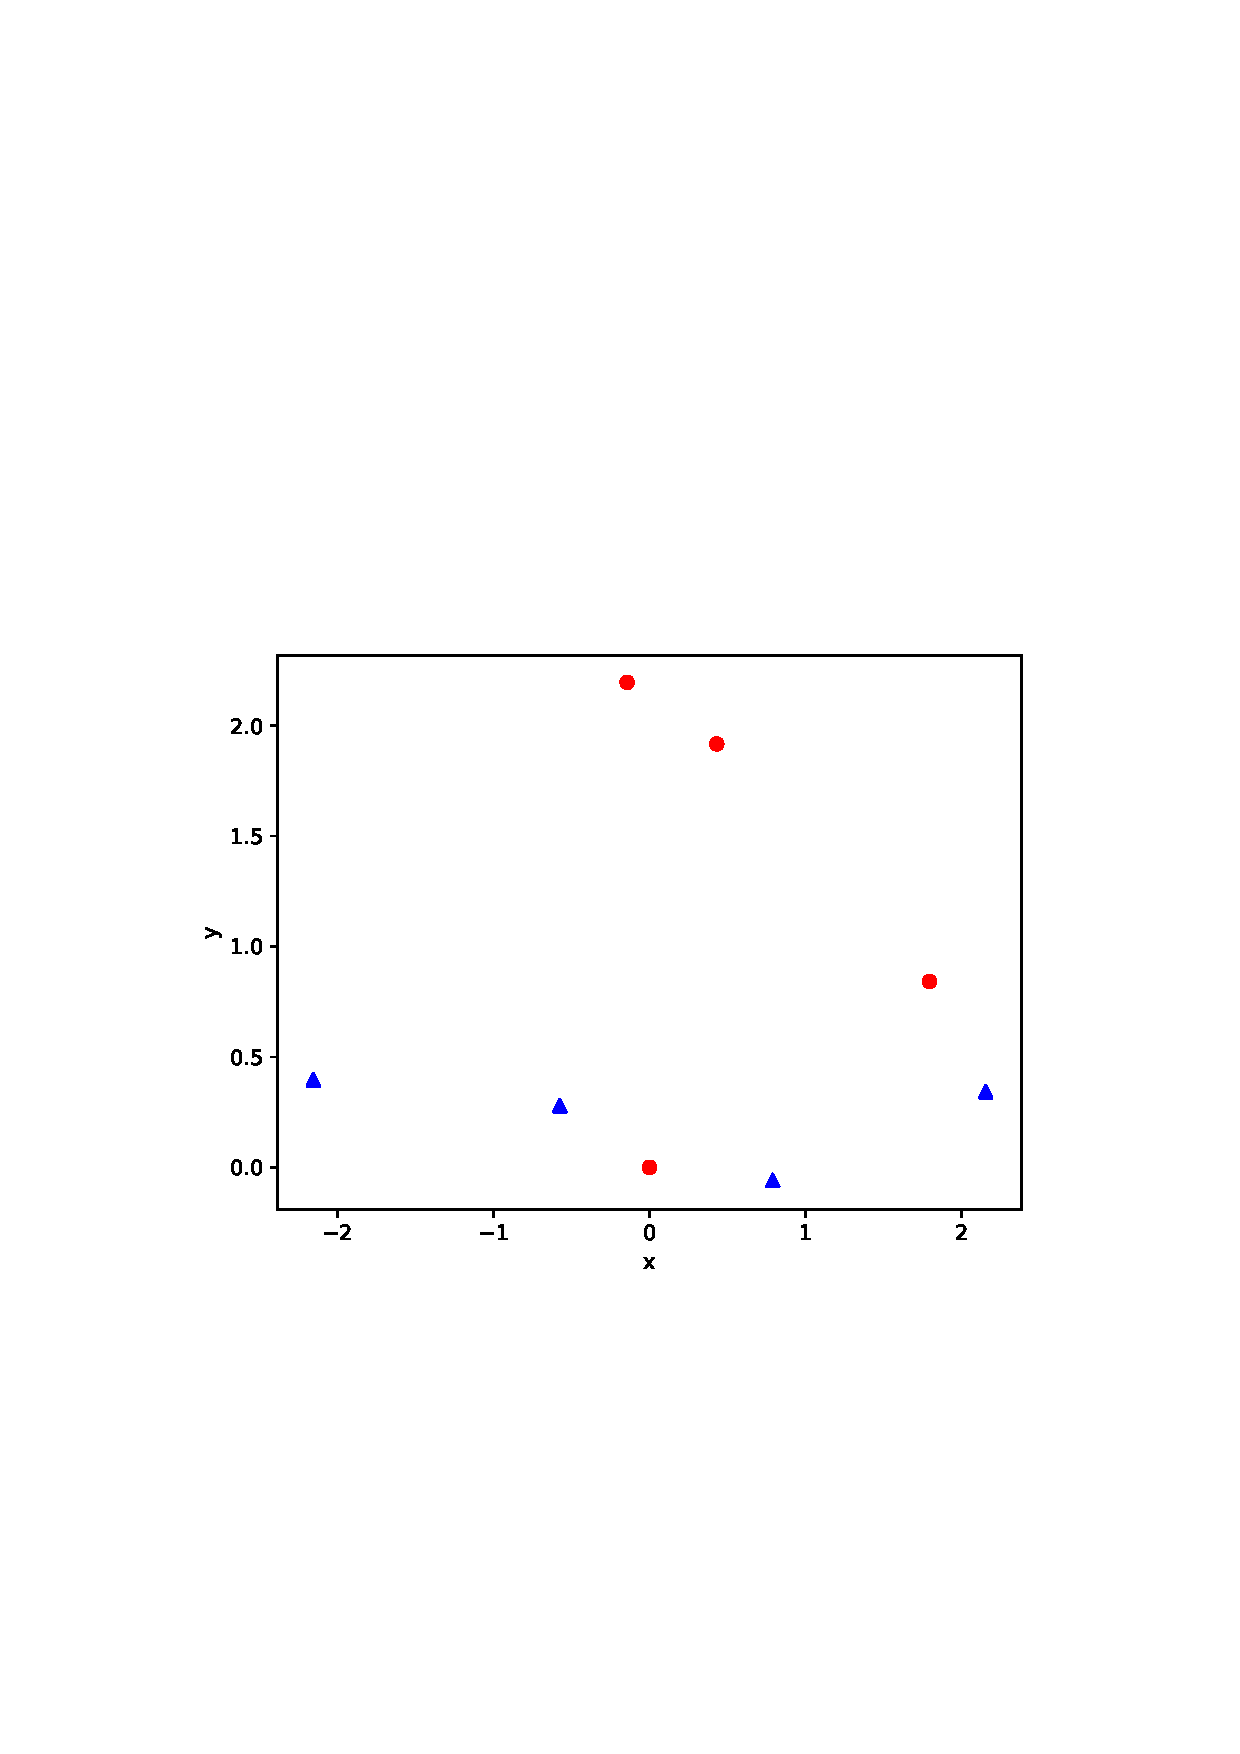
\includegraphics[width = 0.6\textwidth,height=0.3\textheight]{two}
\end{figure} 
降到一维的空间分布
\begin{figure}[H]
	\centering
	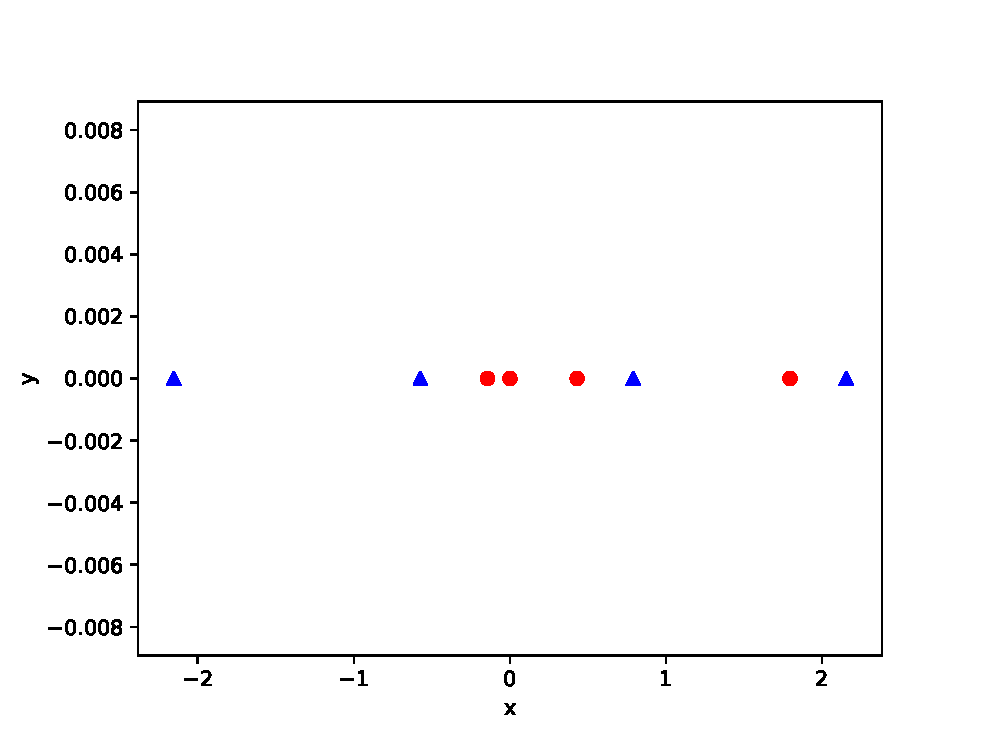
\includegraphics[width = 0.6\textwidth,height=0.3\textheight]{one}
\end{figure} 

\end{document}